\documentclass[aspectratio=169,12pt]{beamer}

\usetheme{CambridgeUS}
\usecolortheme{beaver}
\setbeamertemplate{navigation symbols}{}
\setbeamertemplate{footline}[frame number]

\usepackage{amsmath,amssymb}
\usepackage{tikz}
\usetikzlibrary{calc,angles,quotes,arrows.meta}
\usepackage{booktabs}
\usepackage{listings}
\usepackage{xcolor}
\usepackage{mathtools}

\definecolor{codebg}{RGB}{247,249,251}
\definecolor{coderule}{RGB}{0,100,180}
\definecolor{codekw}{RGB}{0,92,197}
\definecolor{codecmt}{RGB}{90,150,95}
\definecolor{codefn}{RGB}{150,75,20}

\lstset{
  basicstyle=\ttfamily\footnotesize,
  keywordstyle=\color{codekw}\bfseries,
  commentstyle=\color{codecmt}\itshape,
  emph={sign,svd,random_orthogonal,range},
  emphstyle=\color{codefn}\bfseries,
  backgroundcolor=\color{codebg},
  frame=l,
  rulecolor=\color{coderule},
  framerule=2.5pt,
  framesep=8pt,
  xleftmargin=18pt,
  xrightmargin=8pt,
  aboveskip=6pt,
  belowskip=4pt,
  lineskip=1pt,
  showstringspaces=false,
  columns=fullflexible,
  keepspaces=true,
  tabsize=4,
}

\definecolor{acc}{RGB}{180,30,30}
\definecolor{key}{RGB}{0,100,180}
\definecolor{hi}{RGB}{200,80,0}

\title{The Science of Bit-Hashed Retrieval}
\subtitle{SimHash, Asymmetric Quantization, and Why 96 Bytes Beats 3072}
\author{Reading Group}
\date{June 29, 2026}

% ---------------------------------------------------------------
\begin{document}

\begin{frame}
  \titlepage
\end{frame}

% ---------------------------------------------------------------
\begin{frame}{The scale problem}

\begin{columns}
\column{0.55\textwidth}
  You have a corpus of \textbf{50 million documents}.\\[6pt]
  Each is a \textbf{768-dimensional fp32 embedding}.\\[6pt]
  That's $\approx \mathbf{150\,\text{GB}}$ of vectors.\\[14pt]
  At query time you need the top-$K$ closest vectors\\
  to an incoming query — in \textbf{milliseconds}.\\[14pt]
  \onslide<2->{
  Brute-force dot product:\\
  $50\text{M} \times 768 \text{ mults} \approx 38\text{B ops}$ per query.\\[6pt]
  On a modern CPU at 10 GFLOP/s: \textbf{3.8 s per query.}
  }

\column{0.4\textwidth}
  \onslide<3->{
  \centering
  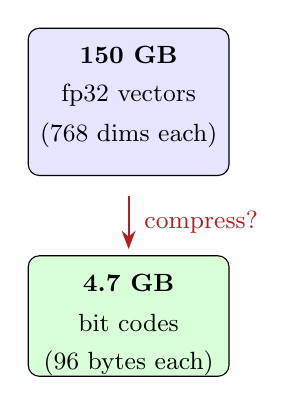
\begin{tikzpicture}[scale=0.85]
    \draw[fill=blue!10,rounded corners=4pt] (0,0) rectangle (3,2.2);
    \node at (1.5,1.8) {\small \textbf{150 GB}};
    \node at (1.5,1.2) {\small fp32 vectors};
    \node at (1.5,0.6) {\small (768 dims each)};
    \draw[-{Stealth},thick,acc] (1.5,-0.3) -- (1.5,-1.1)
      node[midway,right=2pt]{\small compress?};
    \draw[fill=green!15,rounded corners=4pt] (0,-1.2) rectangle (3,-3);
    \node at (1.5,-1.6) {\small \textbf{4.7 GB}};
    \node at (1.5,-2.2) {\small bit codes};
    \node at (1.5,-2.8) {\small (96 bytes each)};
  \end{tikzpicture}
  }
\end{columns}
\end{frame}

% ---------------------------------------------------------------
\begin{frame}{The dream: 32$\times$ compression, near-zero recall loss}

\begin{center}
\begin{tabular}{lrrr}
\toprule
Representation & Bytes/doc & Throughput & Recall \\
\midrule
fp32 (768-dim)    & 3072  & \textit{baseline} & 100\% \\
1-bit codes (768-dim) & 96  & \textbf{2308 M cmp/s} & $\sim$95\%+ \\
2-bit codes (768-dim) & 192 & 70 M cmp/s & higher \\
4-bit codes (768-dim) & 384 & 76 M cmp/s & even higher \\
\bottomrule
\end{tabular}
\end{center}

\vspace{10pt}
\onslide<4->{
\begin{center}
\Large\textbf{But \emph{why} does discarding magnitude work at all?}
\end{center}
}
\end{frame}

% ---------------------------------------------------------------
\begin{frame}{The central question}

\begin{center}
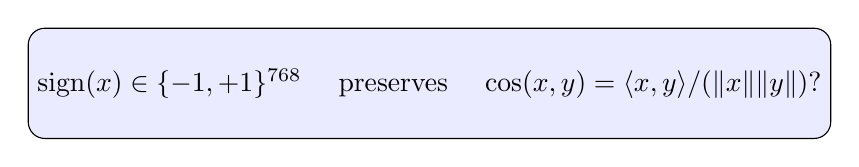
\begin{tikzpicture}
  \node[draw,rounded corners=6pt,fill=blue!8,minimum width=8cm,minimum height=1.4cm]
    at (0,0) {
      $\operatorname{sign}(x) \in \{-1,+1\}^{768}$
      \quad preserves \quad
      $\cos(x,y) = \langle x,y\rangle / (\|x\|\|y\|)$?
    };
\end{tikzpicture}
\end{center}

\vspace{12pt}
\onslide<2->{
The answer is: \textbf{yes, in expectation, via a beautiful geometric argument.}\\[8pt]
It rests on a single identity due to Charikar (2002), building on\\
Goemans--Williamson (1995).\\[8pt]
The argument is \textcolor{acc}{\textbf{dimension-free}}: it works for any $D$.
}
\end{frame}

% ---------------------------------------------------------------
\begin{frame}{One random hyperplane}

Draw a single random hyperplane $h \sim \mathcal{N}(0,I_D)$.\\[4pt]
It partitions $\mathbb{R}^D$ into two half-spaces: $\langle h,v\rangle > 0$ and $\langle h,v\rangle < 0$.\\[8pt]

\begin{columns}
\column{0.55\textwidth}
\textbf{Charikar SimHash bound}:
\[
  \Pr_h\!\bigl[\operatorname{sign}\langle h,x\rangle = \operatorname{sign}\langle h,y\rangle\bigr]
  \;=\; \textcolor{key}{1 - \frac{\theta(x,y)}{\pi}}
\]
where $\theta(x,y) = \arccos\!\bigl(\langle x,y\rangle/(\|x\|\|y\|)\bigr)$.\\[4pt]
\onslide<2->{
Equivalently: $\Pr[\text{disagree}] = \theta/\pi$
— a \textbf{monotone} function of $\cos\theta$.
}

\column{0.42\textwidth}
\onslide<3->{
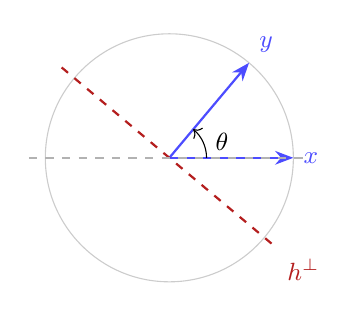
\begin{tikzpicture}[scale=1.05]
  \draw[gray!40] (0,0) circle (1.5);
  \coordinate (O) at (0,0);
  \coordinate (X) at (1.5,0);
  \coordinate (Y) at ({1.5*cos(50)},{1.5*sin(50)});
  \draw[-{Stealth},thick,blue!70] (O) -- (X) node[right]{\small $x$};
  \draw[-{Stealth},thick,blue!70] (O) -- (Y) node[above right]{\small $y$};
  \draw[acc,dashed,thick] ({-1.7*sin(50)},{1.7*cos(50)}) -- ({1.7*sin(50)},{-1.7*cos(50)})
    node[below right]{\small $h^\perp$};
  \draw[gray!60,dashed,thick] (-1.7,0) -- (1.7,0);
  \draw[->] (0.45,0) arc (0:50:0.45) node[midway,right=1pt]{\small $\theta$};
\end{tikzpicture}
}
\end{columns}
\end{frame}

% ---------------------------------------------------------------
\begin{frame}{Why the bound holds: a 3-step proof}

\textbf{Goal}: show $\Pr_h[\operatorname{sign}\langle h,x\rangle \neq \operatorname{sign}\langle h,y\rangle] = \theta/\pi$.

\vspace{4pt}
\begin{enumerate}\setlength\itemsep{2pt}
\item<1-> \textbf{Reduce to 2D.}
  Decompose $h = h_P + h_{P^\perp}$, $P = \operatorname{span}(x,y)$.
  Signs depend only on $h_P \sim \mathcal{N}(0,I_2)$ by rotational invariance.

\item<2-> \textbf{$h_P$ points uniformly on $S^1$.}
  Write $h_P = R\cdot u$; signs depend only on $u$, not the radius $R$.

\item<3-> \textbf{Count the separating arc.}
  The hyperplane $u^\perp$ separates $x$ from $y$ when its direction falls between
  them: two arcs of length $\theta$ each, total $2\theta$ out of $2\pi$.
  \[
    \Pr[\text{disagree}] = \frac{2\theta}{2\pi} = \frac{\theta}{\pi} \qquad \blacksquare
  \]
\end{enumerate}

\onslide<4->{
\vspace{2pt}
\textcolor{hi}{\textbf{Key remark:} The proof never uses $D$. The bound is dimension-free.}
}
\end{frame}

% ---------------------------------------------------------------
\begin{frame}{Geometric picture of the proof}

\begin{center}
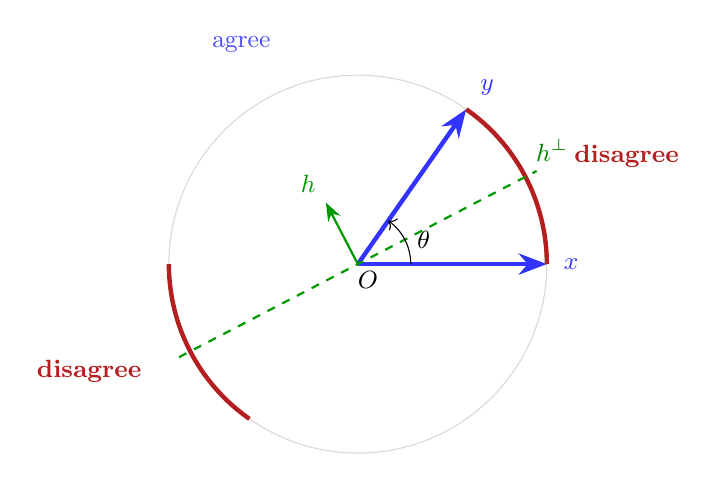
\begin{tikzpicture}[scale=1.6]
  \draw[gray!30] (0,0) circle (1.5);
  \coordinate (O) at (0,0);
  \coordinate (Xv) at (1.5,0);
  \coordinate (Yv) at ({1.5*cos(55)},{1.5*sin(55)});

  % Vectors x and y
  \draw[-{Stealth},ultra thick,blue!80] (O) -- (Xv) node[right=2pt]{\small $x$};
  \draw[-{Stealth},ultra thick,blue!80] (O) -- (Yv) node[above right=1pt]{\small $y$};

  % Red arcs: range of hyperplane h⊥ directions that separate x from y.
  % h⊥ at angle α separates x (at 0°) from y (at 55°) when α ∈ (0°,55°) or (180°,235°).
  \draw[acc,ultra thick] (1.5,0) arc (0:55:1.5);
  \draw[acc,ultra thick] (-1.5,0) arc (180:235:1.5);

  % Example: hyperplane h⊥ at 27.5° (bisecting x and y).
  % h points at 27.5°+90°=117.5° — drawn as a short arrow.
  \draw[green!60!black,dashed,thick]
    ({-1.6*cos(27.5)},{-1.6*sin(27.5)}) -- ({1.6*cos(27.5)},{1.6*sin(27.5)});
  \node[green!50!black,font=\small] at ({1.65*cos(27.5)+0.08},{1.65*sin(27.5)+0.14}) {$h^\perp$};
  \draw[-{Stealth},green!60!black,thick] (O)
    -- ({0.55*cos(117.5)},{0.55*sin(117.5)}) node[above left,font=\small]{$h$};

  % Angle label
  \draw[->] (0.42,0) arc (0:55:0.42) node[midway,right=1pt]{\small $\theta$};

  % Labels — outside the circle (radius 1.5), anchored away from the center
  \node[acc,font=\small\bfseries,anchor=west]
    at ({1.85*cos(27.5)},{1.85*sin(27.5)}) {disagree};
  \node[acc,font=\small\bfseries,anchor=east]
    at ({1.85*cos(207.5)},{1.85*sin(207.5)}) {disagree};
  \node[blue!70,font=\small,anchor=south]
    at ({1.85*cos(120)},{1.85*sin(120)}) {agree};

  \node[font=\small] at (0.08,-0.13) {$O$};
\end{tikzpicture}
\end{center}

\vspace{-4pt}
The \textcolor{acc}{\textbf{red arcs}} mark where the hyperplane $h^\perp$ falls \emph{between} $x$ and $y$.
Each arc has width $\theta$; total fraction = $2\theta / 2\pi = \theta/\pi$.

\end{frame}

% ---------------------------------------------------------------
\begin{frame}{From 1 bit to $D$ bits: Hamming distance as a cosine estimator}

Draw $D$ \emph{independent} hyperplanes $h_1,\ldots,h_D$ and hash:
\[
  x \;\longmapsto\; \bigl(\operatorname{sign}\langle h_1,x\rangle,\;\ldots,\;\operatorname{sign}\langle h_D,x\rangle\bigr)
  \;\in\; \{-1,+1\}^D
\]

\vspace{6pt}
\onslide<2->{
Let $A_w = \mathbf{1}[\operatorname{sign}\langle h_w,x\rangle = \operatorname{sign}\langle h_w,y\rangle]$.
By the bound: $\mathbb{E}[A_w] = 1 - \theta/\pi$.\\[6pt]
By linearity of expectation, the Hamming distance
\[
  H(x,y) = \sum_{w=1}^D (1-A_w)
\]
\textcolor{key}{is an unbiased estimator of $\dfrac{D}{\pi}\cdot\theta(x,y)$.}
}

\vspace{8pt}
\onslide<3->{
\textbf{For the full-precision encoder}: the encoder's weights \emph{are} the random projections
— no extra matrix needed. $\operatorname{sign}(x)$ is the code.
}
\end{frame}

% ---------------------------------------------------------------
\begin{frame}{How noisy is it? (D = 768)}

Each bit $A_w$ is a Bernoulli with $p = 1 - \theta/\pi$.
Since $H \sim \text{Binomial}(D,\, \theta/\pi)$, its standard deviation is:
\[
  \sigma_H \;\approx\; \sqrt{D \cdot p(1-p)}
\]

At a target similarity $\cos\theta \approx 0.9$ (i.e.\ $\theta \approx 26^{\circ}$):
\[
  \sigma_H \;\approx\; \sqrt{768 \times 0.144 \times 0.856}
  \;\approx\; \textcolor{key}{\mathbf{10\;\text{bits}}}
\]

\vspace{2pt}
\onslide<2->{
Hamming distances span $0$ (identical) to $768$ (antipodal), centered near $384$ for
unrelated pairs. \textbf{$\sigma_H = 10$ is small.}\\[3pt]
The gap between a true match ($\cos\theta = 0.9$, $E[H]\approx110$) and a near-miss
($\cos\theta = 0.7$, $E[H]\approx194$)
corresponds to $\approx 84$ bits in Hamming space — well above the noise.\\[3pt]
}
\onslide<3->{
\textcolor{hi}{\textbf{This is why 1-bit codes work for text retrieval.}}\\
The empirical cosine gap between relevant and non-relevant passages is larger
than the estimator's noise floor.
}
\end{frame}

% ---------------------------------------------------------------
\begin{frame}{Is the encoder its own projection? The isotropy problem}

SimHash assumes an \textbf{isotropic Gaussian} projection. A trained encoder is
\emph{not} random --- does skipping $W$ preserve cosine? \textbf{We measured it.}

\onslide<2->{
\textbf{granite-311m, 178k ClapNQ passages} (\texttt{tests/test\_embedding\_isotropy.py}):
\begin{center}\small
\begin{tabular}{lrl}
\toprule
Metric & Value & Ideal \\
\midrule
sign imbalance       & \textcolor{acc}{0.50} & $<0.05$ --- one dim is a \emph{dead} constant bit \\
mean offset          & 0.03 & $<0.05$ \\
effective-rank ratio & \textcolor{acc}{0.21} & $\to 1$ --- uses $\sim$21\% of 768 dims \\
cov.\ spectral ratio & \textcolor{acc}{1465} & $\to 1$ --- variance in a few directions \\
\bottomrule
\end{tabular}
\end{center}
}

\onslide<3->{
\textbf{Strongly anisotropic} with \emph{rogue} dimensions --- naked
$\operatorname{sign}(x)$ wastes bits. Two fixes:
\begin{itemize}\setlength\itemsep{1pt}\small
  \item \textbf{Cheap (affine):} center + per-dim standardize --- fixes sign balance
    ($0.50\!\to\!0.03$); \textcolor{key}{universal win}, no decorrelation (rank $\approx0.21$).
  \item \textbf{Structural:} a rotation $W$ to decorrelate the axes --- \emph{which} $W$? (next)
\end{itemize}
}
\end{frame}

% ---------------------------------------------------------------
\begin{frame}{Choosing the rotation $W$: a menu}

$W \in \mathbb{R}^{d\times D}$ with \textbf{orthonormal rows} (so the fp32 rescore tier stays faithful).

\vspace{4pt}
\begin{center}\small
\begin{tabular}{lccl}
\toprule
Method & Data? & Labels? & Idea \\
\midrule
Identity              & --  & --  & no rotation; bits stay correlated \\
Random orthogonal     & no  & no  & JL / SimHash; unbiased but data-blind \\
PCA / ZCA whitening   & yes & no  & align \& equalize variance; amplifies low-var noise \\
\textbf{ITQ}          & yes & no  & rotate to minimize quantization error (next) \\
Supervised hashing    & yes & yes & similarity-/rank-preserving loss \\
RL + NDCG (REINFORCE) & yes & yes & optimize the metric directly (last) \\
\bottomrule
\end{tabular}
\end{center}

\vspace{6pt}
\onslide<2->{
The axis of choice: \textbf{data-awareness} and \textbf{directness to NDCG} vs.\ \textbf{cost}
and \textbf{label appetite}. Standardize first; then a rotation is the next lever ---
most useful when reducing to $d = D/2$.
}
\end{frame}

% ---------------------------------------------------------------
\begin{frame}[fragile]{ITQ: learn $W$ by minimizing quantization error}

\textbf{Idea} (Gong \& Lazebnik 2011): rotate so the signs sit close to the data.
PCA to $d$ dims ($Z = XP$), then find the orthogonal $R$ minimizing the binary
\emph{quantization error}
\vspace{-4pt}
\[
  \min_{R^\top R = I}\; \bigl\| \operatorname{sign}(ZR) - ZR \bigr\|_F^2 .
\]
\vspace{-10pt}

\textbf{Alternating minimization} --- each step is a closed-form, monotone minimizer:
\begin{lstlisting}[language=Python]
R = random_orthogonal(d)
for _ in range(n_iters):
    B = sign(Z @ R)            # nearest binary codes
    U, _, Vt = svd(B.T @ Z)    # orthogonal Procrustes
    R = Vt.T @ U.T             # R = V U^T minimizes ||B - Z R||
W = (P @ R).T                  # (d, D), orthonormal rows
\end{lstlisting}

\onslide<2->{
\vspace{-3pt}
\small
\textbf{Measured} (SciFact / granite-311m): ties identity at full $d$ with the
\emph{best} Recall@100; at $d{=}D/2$ \textcolor{key}{beats a random rotation by $+0.018$ NDCG}.
Unsupervised, label-free, $\sim$50 passes once at build time.
}
\end{frame}

% ---------------------------------------------------------------
\begin{frame}{Training $W$ for NDCG directly: REINFORCE}

NDCG \emph{and} $\operatorname{sign}(\cdot)$ are both \textbf{non-differentiable} --- so optimize
$W$ with policy-gradient RL, taking \textbf{NDCG itself as the reward}.

\vspace{2pt}
\onslide<2->{
\textbf{Double-orthogonal parametrization} (keeps $W$ on the Stiefel manifold):
\[
  W = U_d\,[\,I_d \;\; 0\,]\,V_D^\top,\qquad
  U_d = e^{A_d}\in SO(d),\;\; V_D = e^{A_D}\in SO(D),
\]
with skew-symmetric generators $A_d, A_D$ ($A^\top = -A$) as the free, unconstrained parameters.
}

\vspace{2pt}
\onslide<3->{
\textbf{Stochastic code policy} $\pi(b_k{=}{+}1\mid x) = \sigma\!\bigl(\beta\,(Wx)_k\bigr)$ ---
sample codes, retrieve, score:
\[
  J = \mathbb{E}_{q,\,B\sim\pi}\!\bigl[\operatorname{NDCG@}K\bigr],\qquad
  \nabla J = \mathbb{E}\bigl[(\operatorname{NDCG} - \bar{b})\,\nabla \log \pi(B)\bigr]
\]
($\bar{b}$ = EMA baseline for variance reduction). Backprop $\nabla\log\pi$ into $A_d, A_D$; ascend.
}

\vspace{2pt}
\onslide<4->{
\textcolor{acc}{\textbf{Caveats:}} high variance, hungry for labeled queries, overfits qrels.
Warm-start from \textbf{ITQ}; use NDCG-RL as a final polish, validated on the recall sweep.
}
\end{frame}

% ---------------------------------------------------------------
\begin{frame}{Symmetric vs. asymmetric: why it matters}

\textbf{Symmetric}: quantize \emph{both} query and database to $b$ bits.\\[2pt]
Per-dimension error: $(q_w{+}\varepsilon_q)(y_w{+}\varepsilon_y) - q_w y_w
= q_w\varepsilon_y + y_w\varepsilon_q + \varepsilon_q\varepsilon_y$\\[1pt]
Leading variance (two additive noise sources):
\[
  \operatorname{Var}[\hat{s}] \;\approx\;
  \frac{\Delta_q^2}{12}\|y\|^2 \;+\; \frac{\Delta_y^2}{12}\|q\|^2
\]

\onslide<2->{
\textbf{Asymmetric (ASH)}: keep query in fp32, quantize only the database.
\[
  \hat{s}_i = \sum_w q'_w \cdot v_{i,w}, \qquad
  \operatorname{Var}[\hat{s}_i] \;\leq\; \|q'\|^2 \cdot \frac{\Delta_b^2}{12}
\]
\textcolor{key}{\textbf{One}} noise source instead of two — factor of $\mathbf{2}$ in variance.
}

\vspace{1pt}
\onslide<3->{
\textbf{The $b=1$ case is more severe.} Quantizing a unit vector to $\pm 1$/dim
inflates its norm to $\sqrt{D}$, collapsing magnitude --- asymmetric avoids this
on the query side.
}
\end{frame}

% ---------------------------------------------------------------
\begin{frame}{The quantization grid $V_b$}

The database dimension $y_w$ is quantized to $b$ bits using the grid:
\[
  V_b = \{2c - (2^b - 1) \mid c = 0,\ldots,2^b - 1\}
\]

\vspace{4pt}
\begin{center}
\begin{tabular}{cll}
\toprule
$b$ & Grid $V_b$ & Level spacing $\Delta_b$ \\
\midrule
1 & $\{-1,\;+1\}$ & 2 \\
2 & $\{-3,\;-1,\;+1,\;+3\}$ & 2 \\
4 & $\{-15,\;-13,\;\ldots,\;+13,\;+15\}$ & 2 \\
\bottomrule
\end{tabular}
\end{center}

\vspace{3pt}
\onslide<2->{
Each vector gets a \textbf{per-vector scale} $s_i = \|y_i\|/\sqrt{d}$, stored as fp16.\\[3pt]
After dividing by $s_i$, the distribution has unit MSE, so the levels straddle the
empirical quartiles with no wasted range.\\[3pt]
\textcolor{key}{The scale costs 2 bytes per code} (0.5\% overhead for $b=4$, $d=768$).
}
\end{frame}

% ---------------------------------------------------------------
\begin{frame}{Under the hood: how it runs fast (the short version)}

\begin{columns}
\column{0.5\textwidth}
\textbf{1-bit (Hamming) kernel:}
\[
  H(q,x) = \sum_{w=0}^{11} \operatorname{popcount}(q_w \oplus x_w)
\]
12 words of 64 bits = 768-bit code.\\
XOR then popcount: \textbf{2 instructions per word}.\\[8pt]
\onslide<2->{
\textbf{Data layout (SoA, not AoS):}\\
Store word $w$ for all $N$ codes contiguously.\\
Enables unit-stride SIMD loads.
}

\column{0.48\textwidth}
\onslide<3->{
\textbf{b-bit asymmetric kernel:}\\
Query stays in fp32.\\
DB codes unpacked via shuffle LUT.\\
Inner product via SIMD FMA.\\[8pt]
\textbf{Query batching trick:}\\
Load each DB word \emph{once},\\
score $NQ=8$ queries against it.\\
Effective bandwidth $\div 8$.
}
\end{columns}

\vspace{5pt}
\onslide<4->{
Top-$K$ is maintained as a \textbf{bounded max-heap on the stack} — threaded through
the scan loop with one integer compare per SIMD block.
}
\end{frame}

% ---------------------------------------------------------------
\begin{frame}{The numbers (50M codes, 32 threads, AVX2 host)}

\begin{center}
\begin{tabular}{lrrl}
\toprule
Kernel & cmp/s & GB/s & Bottleneck \\
\midrule
Hamming top-1 (NQ=8 batched) & \textbf{2308 M} & 27.7 & memory \\
Hamming top-100              & 740 M           & 71.1 & memory \\
Asym $b=1$ (single thread)   & 0.55 M          & 0.1  & FMA unpack \\
Asym $b=2$ (single thread)   & 2.19 M          & 0.4  & FMA \\
Asym $b=4$ (single thread)   & 2.36 M          & 0.9  & FMA \\
\bottomrule
\end{tabular}
\end{center}

\vspace{1pt}
\onslide<2->{
\textbf{Key observations:}
\begin{itemize}\setlength\itemsep{1pt}
  \item Hamming hits the \textbf{DRAM bandwidth wall} at 71 GB/s — can't go faster without an outer index.
  \item Asym $b\in\{2,4\}$ $\times$ 32 threads $\approx$ \textbf{70 M cmp/s} — within 5\% of bandwidth headroom.
  \item $b=1$ asym is slow: AVX2 can't unpack sign bits efficiently. (Fix queued.)
\end{itemize}
}
\end{frame}

% ---------------------------------------------------------------
\begin{frame}{Does it hold on a real corpus? Natural Questions}

\textbf{Setup}: NQ dev ($\sim$270k passages), 2 encoders; fp32 rescore
($\alpha{=}10$) vs.\ \textbf{Milvus FLAT} (exact fp32).

\vspace{2pt}
\begin{columns}
\column{0.54\textwidth}
\centering\small
\textbf{Quality --- NDCG@10}\\[3pt]
\begin{tabular}{l ccc}
\toprule
 & fp32 & $b{=}2$ & 1-bit \\
\midrule
granite-97m \scriptsize(384d)  & 0.576 & 0.576 & 0.575 \\
granite-311m \scriptsize(768d) & 0.607 & 0.607 & 0.607 \\
\bottomrule
\end{tabular}\\[3pt]
{\scriptsize Match@100 within 0.6\% of fp32.}

\column{0.46\textwidth}
\centering\scriptsize
\textbf{Speed (ms/q, 16-conc)}\\[3pt]
\begin{tabular}{l ccc}
\toprule
                                          & Milvus  & $b{=}2$ & 1-bit \\
\midrule
\multicolumn{4}{l}{\textit{AVX-512 (9950X3D)}}\\
97m  (384d)                               & 5.0  & 0.43 & \textbf{\textcolor{key}{0.23}} \\
311m (768d)                               & 11.7 & 0.81 & \textbf{\textcolor{key}{0.40}} \\
\midrule
\multicolumn{4}{l}{\textit{AVX2 (5955WX)}}\\
97m  (384d)                               & 5.1  & 3.76 & \textbf{\textcolor{key}{0.11}} \\
311m (768d)                               & 10.9 & 7.23 & \textbf{\textcolor{key}{0.17}} \\
\bottomrule
\end{tabular}\\[3pt]
{B/doc: 1-bit 48/96, $b{=}2$ 96/192, fp32 1536/3072.}
\end{columns}

\vspace{3pt}
\onslide<2->{\small
\textcolor{hi}{\textbf{Quality holds for all modes.}} \textbf{1-bit Hamming + fp32 rescore is fastest \emph{and} smallest} --- lossless at 768d. ISA matters: see next slide.
}
\end{frame}

% ---------------------------------------------------------------
\begin{frame}{Hardware portability: AVX-512 vs.\ AVX2}

{\small Same code, two CPUs, identical 16-conc harness. Quality identical (lossless rescore).}

\vspace{2pt}
\begin{center}\scriptsize
\renewcommand{\arraystretch}{0.92}
\begin{tabular}{l c cc c}
\toprule
Mode (dim)                  & B/doc & 9950X3D (AVX-512) & 5955WX (AVX2) & ratio \\
\midrule
Milvus FLAT, 384d           & 1536  & 5.0  & 5.10  & 1.0$\times$ \\
Milvus FLAT, 768d           & 3072  & 11.7 & 10.90 & 0.9$\times$ \\
asym $b{=}2$, 384d          & 96    & 0.43 & 3.76  & 8.7$\times$ \\
asym $b{=}2$, 768d          & 192   & 0.81 & 7.23  & 8.9$\times$ \\
\textbf{1-bit}, 384d        & \textbf{48} & 0.23 & \textbf{\textcolor{key}{0.11}} & \textbf{0.5$\times$} \\
\textbf{1-bit}, 768d        & \textbf{96} & 0.40 & \textbf{\textcolor{key}{0.17}} & \textbf{0.4$\times$} \\
\bottomrule
\end{tabular}
\end{center}

\scriptsize
\onslide<2->{\textbf{Milvus FLAT is ISA-blind} — memory + RPC bound; the 5955WX's 8-ch DDR4 narrowly beats 2-ch DDR5.\par}
\onslide<3->{\textbf{Asym $b{=}2$ collapses on AVX2}: no \texttt{vpmultishiftqb} (VBMI), scalar unpack stalls FMA. Single-thread 768d: 13\,ms (AVX-512+Lever-1) vs 134\,ms (AVX2).\par}
\onslide<4->{\textbf{1-bit is \emph{faster} on AVX2}: \texttt{popcnt}+\texttt{xor} is memory-bound, and this box has more bandwidth.\par}

\vspace{2pt}
\onslide<5->{\small\textcolor{hi}{\textbf{Takeaway:}} asym/1-bit ratio: $\sim$2$\times$ on AVX-512, \textbf{$\sim$42$\times$ on AVX2}. \textcolor{acc}{Deployment default flips with the ISA.}}
\end{frame}

% ---------------------------------------------------------------
\begin{frame}{Open questions: what Plan 3 will answer}

\begin{center}
\begin{tabular}{ll}
\toprule
Scientific question & Experiment \\
\midrule
Does asym $b=2$ match $b=1$ + fp32 rescore at same byte budget? & R0 vs.\ R3 \\
Does halving $d$, doubling $b$ win under random-orthogonal $W$? & R3 vs.\ R4 \\
Is $b=4$ at $d/2$ a Pareto move vs.\ $b=2$ at $d$? & R3 vs.\ R5 \\
How much fp32-baseline NDCG do bit codes sacrifice? & R6 \\
\bottomrule
\end{tabular}
\end{center}

\vspace{6pt}
\onslide<2->{
\textbf{The headline:} \textcolor{acc}{Does asymmetric multi-bit replace \emph{binary + rescore}?}\\[4pt]
If yes: deployment recommendation across the embedding fleet flips.\\
If no: learned projection (v2) becomes the next research lever.
}
\end{frame}

% ---------------------------------------------------------------
\begin{frame}{Summary}

\begin{enumerate}
  \setlength\itemsep{4pt}
  \item \textbf{SimHash} (Charikar 2002): $\Pr[\text{agree}] = 1 - \theta/\pi$ —
    proved by counting a disagreement arc. Dimension-free.

  \item \textbf{$D$ bits $\Rightarrow$ Hamming $\approx$ cosine.}
    Noise $\sigma \approx 10$ bits at $D=768$ — below the relevant/non-relevant gap.

  \item \textbf{The encoder does the projection for free.}
    No random $W$ needed; trained embeddings already project semantic space.

  \item \textbf{Asymmetric beats symmetric.}
    One $O(\Delta^2)$ noise source vs.\ two (plus a symmetric-only $O(\Delta^4)$ cross term):
    $\approx 2\times$ lower variance at leading order, and no magnitude collapse on the query.

  \item \textbf{Speed}: 2308 M cmp/s, 27.7 GB/s — at the DRAM bandwidth ceiling.

  \item \textbf{Open}: does multi-bit asymmetric make binary + rescore obsolete?
\end{enumerate}

\end{frame}

% ---------------------------------------------------------------
\begin{frame}{Discussion}

\begin{columns}
\column{0.5\textwidth}
\textbf{Questions to consider:}
\begin{itemize}
  \item Is the encoder-as-projection argument empirically verified or just plausible?
  \item The $\sigma \approx 10$ bits noise — does it compound when re-ranking?
  \item Asymmetric b=1 is provably suboptimal on AVX2. Does it matter in practice?
  \item Plan 3 recipe sweep assumes BEIR. Retrieval vs.\ RAG use-case differences?
\end{itemize}

\column{0.48\textwidth}
\textbf{Paper:}\\
\textit{simdq Plan 1 — The Science of Bit-Hashed Retrieval}\\
DocUVerse \texttt{simdq} engine, 2026.\\[8pt]
\textbf{Key references:}\\
{\small
Charikar (2002) — SimHash bound\\
Goemans \& Williamson (1995) — hyperplane rounding\\
Tepper \& Willke (2026) — ASH framework\\
Mula, Kurz \& Lemire (2018) — AVX2 popcount
}
\end{columns}

\end{frame}

\end{document}
